% !TeX root = main.tex

\section{实验步骤}

\subsection{制备掺与不掺粉煤灰的水泥净浆试块}

\subsubsection{}
按照实验方案, 固定水灰比为 \num{0.4}, 粉煤灰掺量采用 \qtylist{0; 15; 30}{\percent} 取代水泥, 制备 3 组水泥净浆试块, 每组 3 组试块, 尺寸为 \qtyproduct{40 x 40 x 40}{\milli\meter}.
试件成型 \SI{24}{\hour} 后拆模, 将其放入标准养护室中养护 \SI{7}{\day} 后测试其抗压强度.
\begin{table}[!t]
    \centering
    \caption{水泥试块的配合比}
    \begin{tabular}{|c|c|c|c|c|c|}
    \hline
    实验编号 & 粉煤灰掺量 & 水胶比 & 水泥(g) & 水(g) & 粉煤灰(g) \\ \hline
    1    & 0      & 0.4 & 700   & 280  & 0      \\ \hline
    2    & 15\%   & 0.4 & 595   & 280  & 0.5    \\ \hline
    3    & 30\%   & 0.4 & 490   & 280  & 210    \\ \hline
    \end{tabular}
\end{table}
\han{上面那张图没看懂,我理解是加入0.5ml消泡剂以消除混凝土表面多孔现象,后面的数据是上面的水泥、水、粉煤灰添加量保留两位小数?}
\begin{figure}
    \centering
    \caption{实验数据记录表}
    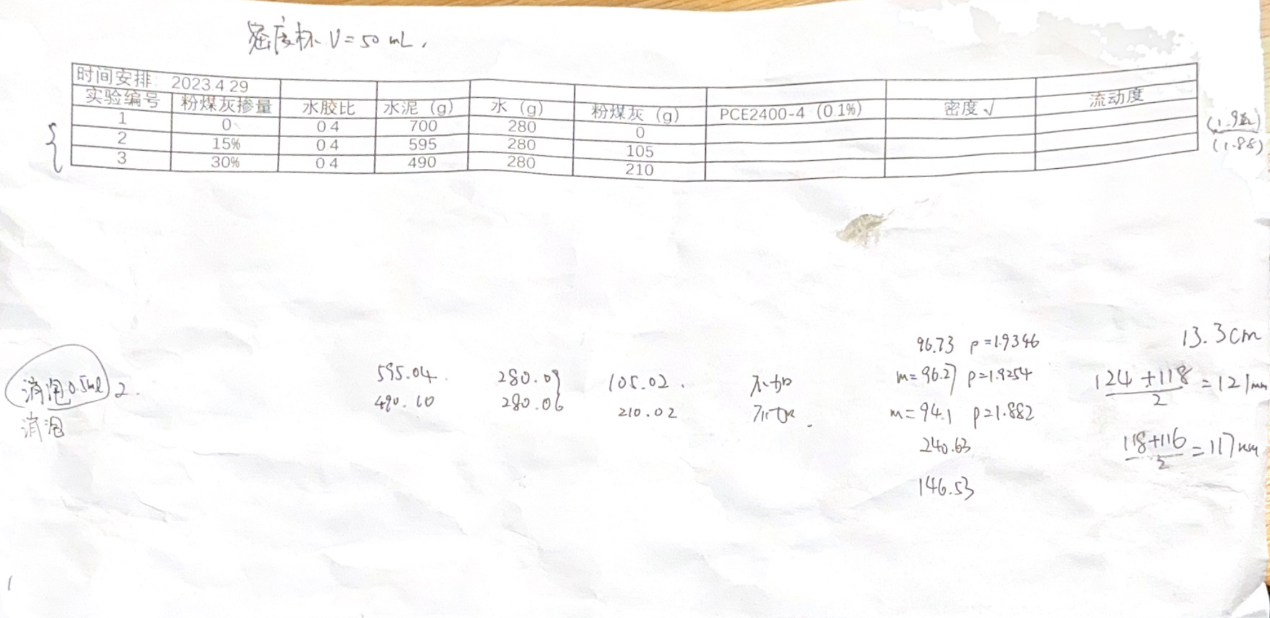
\includegraphics[width = 0.7 \linewidth]{figures/exp1/record table.png}
\end{figure}

\begin{figure}
    \centering
    \caption{浆体流动性实验}
    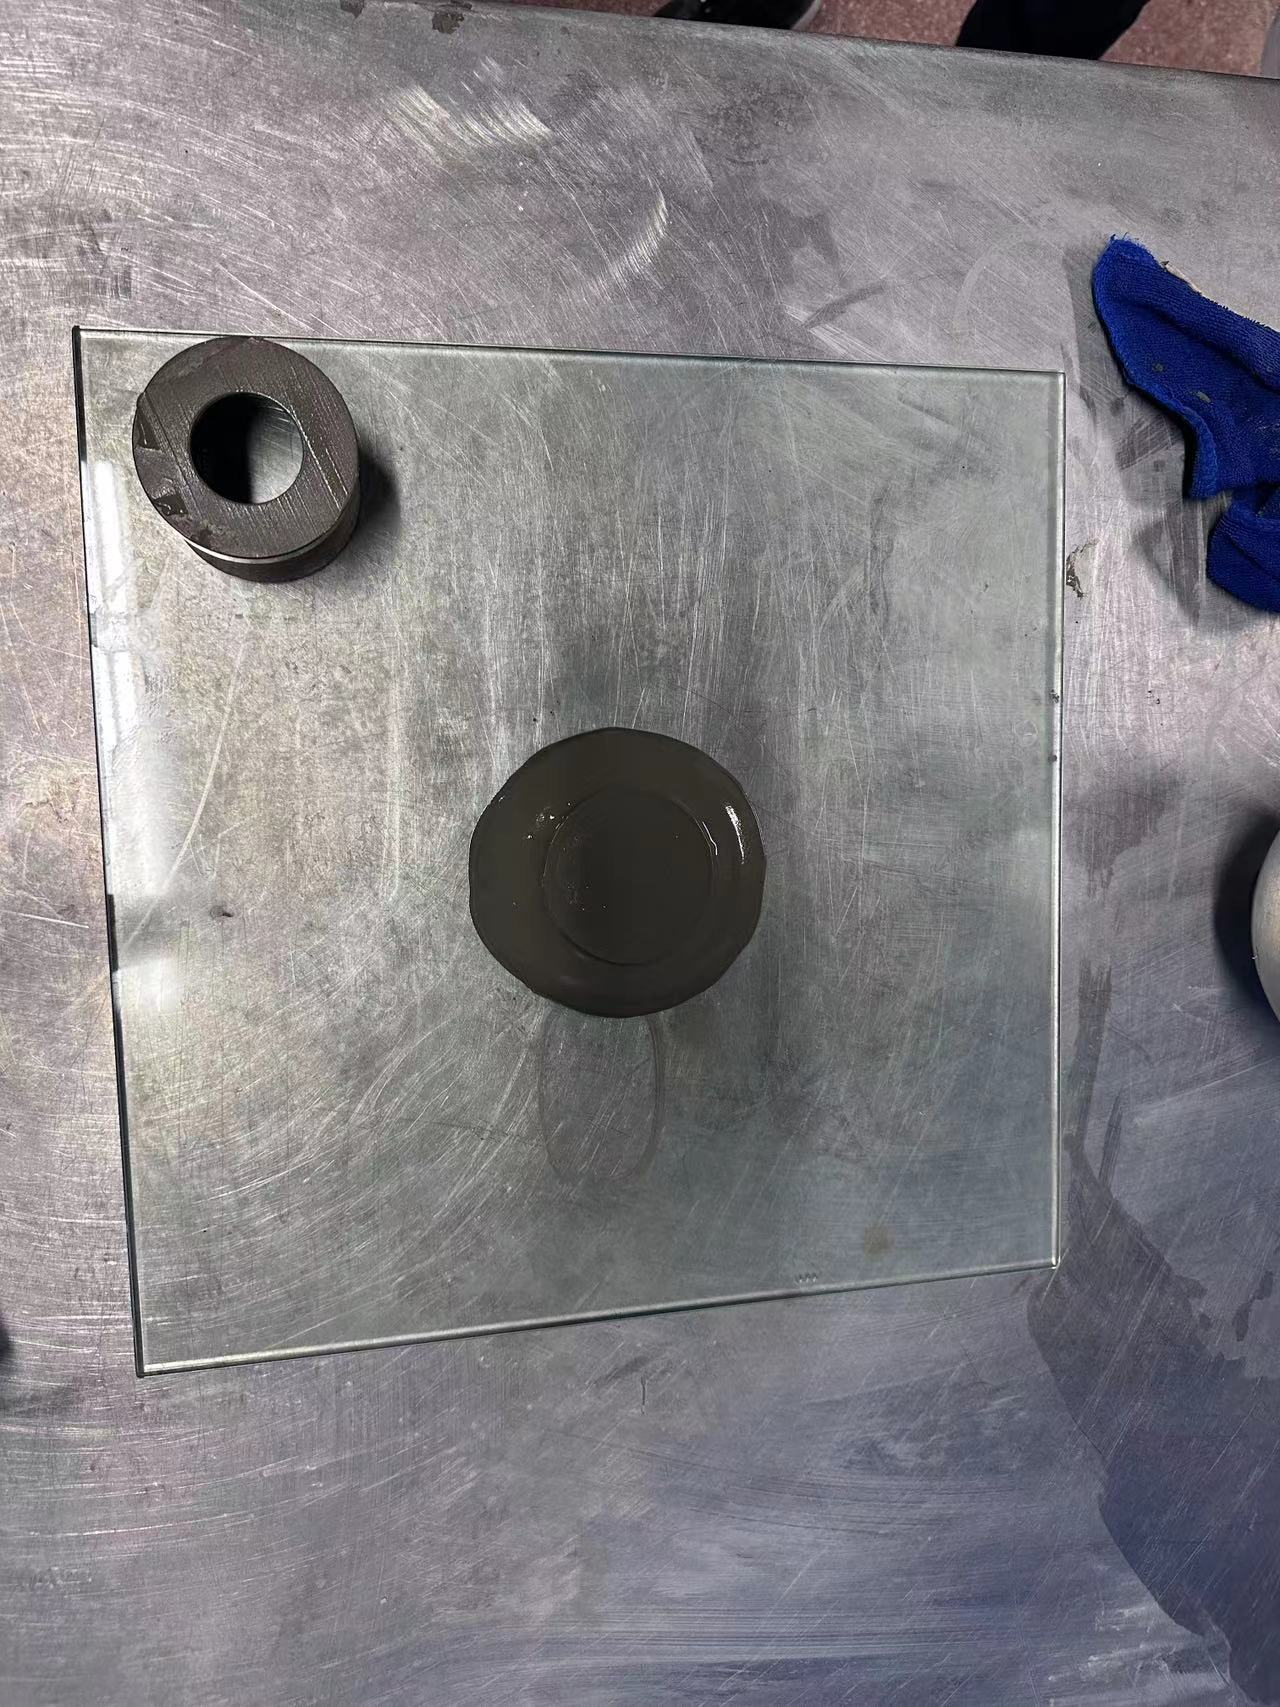
\includegraphics[width = 0.6 \linewidth]{figures/exp1/mobility.png}
\end{figure}

\subsubsection{}
试件成型24h后拆模,将其放入标准养护室中养护7d后测试其抗压强度。
使用试金300kN试验机进行水泥净浆试块抗压强度试验。该试验机最大荷载为300kN,最大位移为200mm。
实验过程中应严格遵照试验机操作规程:
\begin{enumerate}[wide, labelwidth=!, labelindent=0pt]
    \item 开动试验机之前,先确保上下承压板之间无夹具和试样;
    \item 启动计算机;
    \item 启动计算机中的试验机测控软件;
    \item 按下油源面板上的“电源开”、“油泵开”按钮;
    \item 使用试验机测控软件的“砂浆抗压试验”控制模式,将养护7d的各组40 mm*40mm*40mm水泥净浆试块置于试验机上,进行试验;
    \item 测试完成后,按下油源面板上的“油泵关”、“电源关”按钮;
    \item 关闭试验机的测控软件,再关闭计算机!
    \item 将测试用夹具从上下承压板之间取出;
    \item 将废试样带走,将试验机周边清理干净。
\end{enumerate}

设备使用过程中,如出现任何非预期现象,应立即按下油源面板上的“急停”按钮,停止试验机运行!
试验结果如下表所示。(缺少了2-1 2-1的数据,是不是当时少拍了?)
\begin{table}[!t]
    \centering
    \caption{抗压强度测试结果}
    \begin{tabular}{|c|c|}
    \hline
    试样编号 & 抗压强度(MPa) \\ \hline
    1-1  & 39.2      \\ \hline
    1-2  & 36.5      \\ \hline
    3-1  & 30.6      \\ \hline
    3-2  & 30.7      \\ \hline
    \end{tabular}
\end{table}

\subsection{通过 SEM 观察水泥净浆试块断面的微观形貌}

将水泥净浆试块在标准养护室养护至 \SI{7}{\day} 之后, 一部分直接取断面观察其微观形貌.
方法如下: 取试块中央部分制成黄豆粒大小, 并在异丙醇中浸泡 \SI{24}{\hour} 以终止水化; 对随后取出置于 \SI{40}{\degreeCelsius} 的真空烘箱中烘干 \SI{24}{\hour}, 之后对样品进行喷金处理, 最后置于 SEM 下观察其微观形貌.

\subsection{观察抛光样品的背散射电子成像}

将水泥净浆试块在标准养护室养护至 \SI{7}{\day} 之后, 取另一部分水泥净浆样品浸泡在异丙醇中以终止水化, 然后在 \SI{40}{\degreeCelsius} 的真空烘箱中烘干 \SI{24}{\hour}, 之后取出将其嵌入环氧树脂中进行抛光处理.
之后对样品进行喷金处理, 最后置于 SEM 下观察其背散射电子成像.
